%%%%%%%%%%%%%%%%%%%%%%%%%%%%%%%%%%%%%%%%%%%%%%%%%%%%%%%%%%%%%%%%%%%%%%%%%%%
%
% Template for a LaTex article in English.
%
%%%%%%%%%%%%%%%%%%%%%%%%%%%%%%%%%%%%%%%%%%%%%%%%%%%%%%%%%%%%%%%%%%%%%%%%%%%

\documentclass[12pt]{article}

% AMS packages:
\usepackage{amsmath, amsthm, amsfonts}
\usepackage{setspace}
\usepackage{url}
\usepackage{graphicx}
\usepackage{float}
\usepackage{multicol}
% Theorems
%-----------------------------------------------------------------
\newtheorem{thm}{Theorem}[section]
\newtheorem{cor}[thm]{Corollary}
\newtheorem{lem}[thm]{Lemma}
\newtheorem{prop}[thm]{Proposition}
\theoremstyle{definition}
\newtheorem{defn}[thm]{Definition}
\theoremstyle{remark}
\newtheorem{rem}[thm]{Remark}

% Shortcuts.
% One can define new commands to shorten frequently used
% constructions. As an example, this defines the R and Z used
% for the real and integer numbers.
%-----------------------------------------------------------------
\def\RR{\mathbb{R}}
\def\ZZ{\mathbb{Z}}

% Similarly, one can define commands that take arguments. In this
% example we define a command for the absolute value.
% -----------------------------------------------------------------
\newcommand{\abs}[1]{\left\vert#1\right\vert}

% Operators
% New operators must defined as such to have them typeset
% correctly. As an example we define the Jacobian:
% -----------------------------------------------------------------
\DeclareMathOperator{\Jac}{Jac}

%-----------------------------------------------------------------
\title{Overuse of private healthcare insurance services after the Covid-19 pandemic}
\author{David Mori\~na$^{*,1}$, Amanda Fern\'andez-Fontelo$^2$, Montserrat Guill\'en$^1$}
\doublespacing
\begin{document}
\maketitle

\abstract{PER FER.}

\section{Introduction}\label{intro}
Until 2020, the impact of a pandemic on health insurance was recognized as a potential catastrophic risk that could impact claims frequency and severity. It was expected that a pandemic would increase the cost of health insurance. 
After COVID-19 stoke in 2020, some lessons have been learned. The pandemic has caused unprecedented disruption to the global health insurance market, but the reaction is somehow different depending on the country. In the US, health insurance companies have suffered financially due to the pandemic, with many reporting financial losses, including increased claims and decreased premium collections. Because the pandemic has also caused a decrease in the number of people enrolling in health insurance plans. This is due to job loss and reduced income, as well as changing health insurance regulations. As a result, many health insurance companies have been forced to reduce costs, including reducing coverage and raising premiums, which in turn has caused a decrease in the number of people receiving health insurance coverage.
In some other countries, especially those with a marked dual public-private health system the effect on private health insurance was unexpected. The pandemic caused many people to stay home, the number of medical appointments, hospital admissions, and other medical services decreased. This, in turn, led to a decrease in health insurance claims. The decrease in claims was also due to the postponement of elective medical procedures, such as surgeries and other invasive treatments, which are typically covered by health insurance. These procedures were often put on hold due to the strain on healthcare systems, as well as the restrictions on movement in many areas. As a result, the number of claims related to these procedures decreased significantly. Finally, the fear of contracting COVID-19 in healthcare settings led some people to avoid seeking medical care, even for serious conditions that would typically require coverage from health insurance. This also contributed to the decrease in health insurance claims. Overall, the decrease in health insurance claims during the pandemic can be attributed to a combination of factors and a rebound once the pandemic passed was also expected.
Many insurers realized that 2020, 2021 and 2022 were special years in health insurance and actuaries are puzzled about the long-term effects of claiming records. The main problem is to identify whether the fluctuations of claims frequency and severity are back to a stable level after three years, whether immediate health insurance pricing can be resolved by discarding these three years, or whether at least 2022 could be taken as representative for establishing rates in the near future. A tool for correcting the claiming information based on a quantitative assessment of the underreporting/overreporting of claims could be of most interest in order to base future pricing on the most recent years instead of resorting to 2019.

We propose a method to cover these three objectives: 1) identification of the time series of claims breaking points, 2) quantification of the size of the pandemic impact on claiming frequency and 3) a test to decide if the claim frequency series still shows some impact. 

We illustrate our method with data from a Spanish private health insurance company. This firm was affected by the enforcement of ocial distance measures adopted as in many other countries that actually caused a sudden decrease in the health insurance frequency of claims and the decrease was substantial due to the fact that during lockdowns citizens reduced their normal activities and cancelled preventive medical visits, while medical services were mostly dedicated to the COVID-19. Simultaneouly, their postfolio grew substantially as in other European countries, something that is explained by the existence of a saturated public health system which worried many citizens who thought that they should underwrite a private health insurance on top of access to public health to protect them and their families in case of a global mediacl service collapse. Although private hospitals which are accessible for holders of a health insurance contract were also relatively saturated during the pandemic, COVID-19 mainly stroke public hospitals. In general, in these countries, private health insurance plans have boosted and the market expanded with more expensive premiums and many more policyholder than ever before.
The reason why premiums increased even if the initial effect of COVID-19 was a claim reduction is that the pandemic has changed the way health insurance companies approach risk after a merely potential risk event became a realized catastrophic event. Many insurers have taken a more cautious approach to risk, leading to increased premiums, increased deductibles, and decreased coverage. In addition, some insurers have changed their eligibility criteria and are now charging higher premiums for those with pre-existing conditions. The pandemic has also caused an increase in the cost of health care services. This is due to higher demand for services, increased costs for medical supplies, and increased costs for delivering care. As a result, many health insurance companies have reacted with a change in prices that is attributable to a higher uncertainty of a possible increase of claims due to the fact that some pathologies that could have been diagnosed, were not and then the treatment would cost more than what would be expected had they been identified at early stages. Some studies on the long-term effects of COVID-19 in some patients, has also increase the fear of a durable increased level of claims. 
Our main question is to find a way to quantify the effect of the pandemic outbreaks on the time series of claims, by identifying their size in the beginning of the series and their return to a pre-pandemic level after two years. Our method aims to design a step by step procedure that would help health insurers decide when their portfolio information is still affected by the pandemic shock, so that the claiming data is already suitable for predictive modelling, or, in case data are still showing some post-pandemic effect, what is the size of the distortion, and how can the data be corrected for a predictive modelling use.
Overall, the decrease in health insurance claims during the pandemic can be established in more than 20\%.

\subsection{Predictive models}\label{predmodels}
Predictive modeling is a powerful tool used in health insurance rate making that can help insurers better understand risk and price policies more accurately. Predictive models use historical data to identify patterns and predict future behavior. By incorporating predictive models, insurers can better understand the relationship between risk factors and claim costs, and use these results to set appropriate prices for their policies. Predictive models are used in health insurance rate making to identify the most significant factors that determine claim costs and to calculate the expected cost for a policy. Models typically account for several factors, such as age, gender, health status, and past claims history. By analyzing these factors, insurers can better understand the relationship between risk factors and claim costs and set more accurate prices. Additionally, predictive models can be used to identify and adjust for differences between individuals and groups. For example, if a certain group of individuals have a higher likelihood of making a claim, insurers can adjust the price of their policies accordingly. This can help ensure that individuals are not overcharged based on their risk characteristics. Overall, predictive models can be a valuable tool for health insurance rate making. By incorporating predictive models, insurers can better understand the relationship between risk factors and claim costs, and use these results to set more accurate prices for their policies. This can help ensure that individuals are not overcharged based on their risk characteristics, and can also help insurers better understand their risk exposure and adjust their policies accordingly.
The most commonly used predictive models in health insurance rate making are logistic regression, Cox regression, and decision trees. Logistic regression is used to predict whether a person is likely to have a health condition, or the probability of a health event occurring. Cox regression is commonly used to estimate the risk of an event occurring within a given period of time, such as the probability of a person developing a certain condition in the future. Decision trees are used to predict the probability of a health event occurring given a certain set of conditions. These models are used to help inform the rate making process, as they provide insight into the likelihood of certain health events occurring.

The data needed to estimate predictive models and price health insurance will vary depending on the type of health insurance being written. Generally, data should include information on health risks, such as age, gender, health status, pre-existing conditions, and lifestyle choices. Additionally, data on the cost of health care services and the claims history of the insurer should be included. Depending on the type of health insurance being written, other data may be necessary, including data on the health care system, the local economy, and the availability of health care services.

\section{Methods}\label{methods}
This paper proposes an approach adapting the well-known difference-in-differences methodology to the time series setting by explicitly modelling the counterfactual of a time series observed both before and after the occurrence of an event of interest, potentially impacting the evolution of the process as the Covid-19 pandemic in this case. provides a fully Bayesian time-series estimate for the effect; and it uses model averaging to construct the most appropriate synthetic control for modelling the counterfactual. This methodology is also capable of providing accurate forecasts, as shown in the next Section. The performance of this approach is compared to usual time series modelling as ARIMA.
All coding was done in R software (\cite{r_core_team_r_2019}), using the packages \textit{bsts} (\cite{scott_predicting_nodate}) and \textit{CausalImpact} (\cite{brodersen_inferring_2015}).

\subsection{Data}\label{data}
The weekly number of medical claims associated to a private health insurance from one of the biggest companies in Spain, by type of service, province, sex and age group. The overall monthly number of contracts was also taken into account, to control for observed trends unrelated to pandemic consequences. To make the latter weekly, a linear interpolation process was performed. The immediate impact of the Covid-19 pandemic is quantified by comparing the number of claims in the years 2019 and 2020, while the medium and long term consequences are quantified by comparing the number of claims in the years 2019 and 2021. In order to illustrate the ability of the proposed methodology to quantify the impact of the pandemic over the usage of private health services, the next section describes in detail the evolution of medical claims globally, by sex, among people over 60 years old and in the three provinces with largest Spanish cities (Madrid, Barcelona and Valencia). Additionally, some particular services of special interest are also analyzed.

In the supplementary material two different scenarios are considered regarding the definition of the post-pandemic period to be compared with the regular period (2019-01-01 to 2020-03-13) and the pandemic period (2020-03-14 to 2020-06-21). The first approach to the post-pandemic period definition (labeled as scenario 1 in the figures and tables) is to compare the period 2019-01-01 to 2020-06-21 against the period 2020-06-22 to 2021-12-31. The second approach (labeled as scenario 2 in the figures and tables) is to exclude the pandemic period, comparing the period 2019-01-01 to 2020-03-13 against 2020-06-21 to 2021-12-31. 

All the R code used to generate the results and figures described in the next section are available in the GitHub repository \url{http://www.github.com}. TODO: Explicar que les dades no poden ser publicades per restriccions del propietari.

\section{Results}\label{results}
Although a very simplistic approach to quantifying the impact of the Covid-19 pandemic over the usage of health insurance associated services could be just to describe the reduction produced in 2020 respect 2019 and the growth observed in 2021 also respect 2019, it would be complicated to use this information to forecast the future behavior of the number of claims. In our context, we could just say that in 2019 a total number of 11,754,419 claims were observed, for 10,305,088 in 2020 and 13,337,053 in 2021. That means that a decrease of 12\% was observed in 2020 and an increase of around 13\% was produced in 2021. However, it is not possible to go any further from here. A more sophisticated approach that would allow us to get a forecast of the future behavior can be the classical ARIMA time series models, ignoring the fact that the original series is not stationary (Kwiatkowski–Phillips–Schmidt–Shin test p-value of 0.01) and is not clear how to make it stationary using the Box-Jenkins methodology. Fitting the best ARIMA model according to the Akaike's Information Criterion (AIC) to the period January 2019 to June 2021, which is an AR(1), the produced forecast for the period July 2021 to December 2021 is shown in Figure~\ref{fig1}. 

\begin{center}
  \begin{figure}[H]
    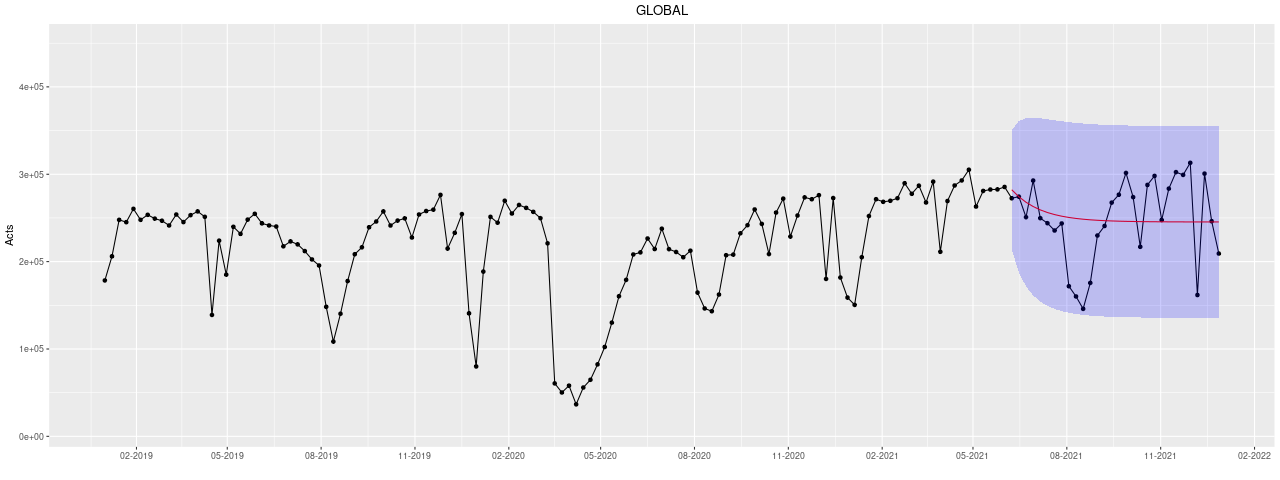
\includegraphics[width=9cm]{Results/arima_global_prediction.png}\caption{Number of weekly claims and ARIMA forecast for the period July-December 2021.}
  \end{figure}\label{fig1}
\end{center}

It can be seen that the ARIMA based forecast is only capable of getting the mean of the process, but at the price of large discrepancies between observed and forecasted values (root mean squared error (RMSE) of 46,989 and mean absolute percentage error (MAPE) of 17.23\%). The forecast fore the same period provided by the proposed approach is shown in Figure~\ref{fig2}.

\begin{center}
  \begin{figure}[H]
    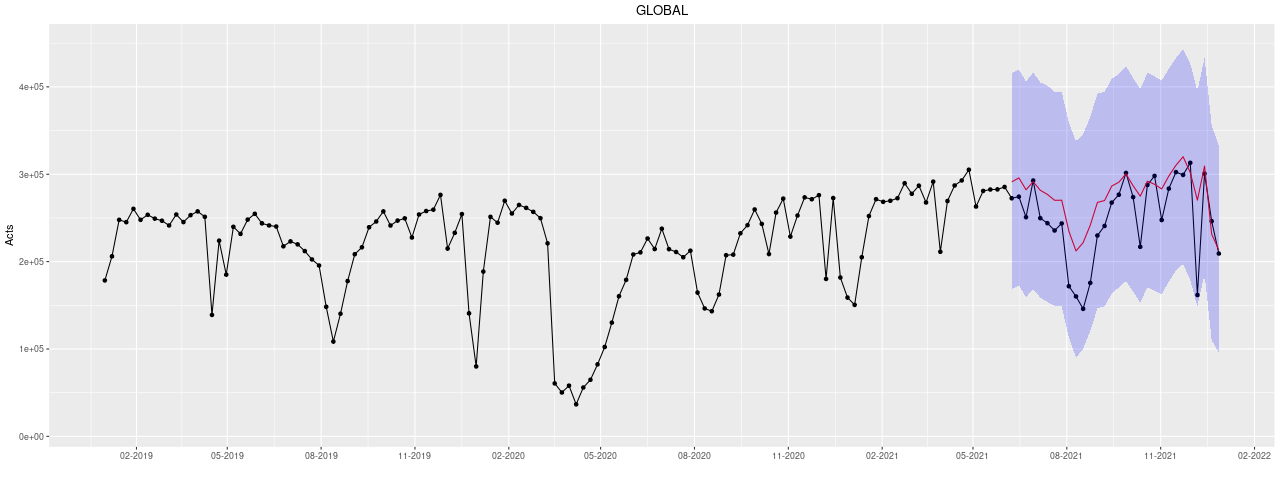
\includegraphics[width=9cm]{Results/bsts_global_prediction.png}\caption{Number of weekly claims and BSTS forecast for the period July-December 2021.}
  \end{figure}\label{fig2}
\end{center}

It is clear from Figure~\ref{fig2} that the forecast produced by the proposed approach is much more accurate than that provided by the classical approach. In this case, the RMSE is around 37,983 and the MAPE is around 14.21\%, in both cases lower than the previous approach. 

\begin{table}[H]\caption{Estimated impact of COVID pandemic and post-pandemic over the usage of health insurance associated services.}
  \centering  
  \begin{tabular}{ccc|cc}
    \hline
    & \multicolumn{2}{c|}{2019-2020} & \multicolumn{2}{c}{2019-2021} \\
    \hline
    & Difference (95\% CI) & p-value & Difference (95\% CI) & p-value\\
    \hline
    Total & X & X & X & X\\
    \hline
    Females & X & X & X & X\\
    Males & X & X & X & X\\
    \hline
    Over 60 & X & X & X & X\\
    \hline
    Oncology & X & X & X & X\\
    Cardiology & X & X & X & X\\
    Obstetrics & X & X & X & X\\
    Urology & X & X & X & X\\
    General medicine & X & X & X & X\\
    Osteopathy & X & X & X & X\\
    \hline
    Madrid & X & X & X & X\\
    Barcelona & X & X & X & X\\
    Valencia & X & X & X & X\\
    \hline
\end{tabular}
\end{table}

\section{Discussion}\label{discussion}
The proposed approach is capable of estimating the impact of the Covid-19 pandemic in the usage of services associated to private health insurances. On one hand, it is shown that a remarkable decrease is observable by the period 2020-03-14 to 2020-06-21, attributable to the mandatory lockdown decreed by the Spanish government, regardless of the specific service or geographic area. On the other hand, and more interestingly, this model can also estimate the posterior impact due to Covid-19 pandemic consequences, that can be translated as an increase in the usage in general (18\% or 10\% of overuse compared to a normal period depending on the scenario), less clear when looking at specific services or geographic areas, probably because the increase is more subtle than the decrease during the lockdown and the time series is too short. In this sense, it would be very interesting to analyze the behavior of the series when more recent data become available.

From the insurance companies point of view, the proposed methodology offers a very convienent alternative to pricing their products on the basis of realistic estimations, overcoming the most common approach to the date, which is simply to ignore the year 2020 and therefore overlooking the posterior overuse of health services due to the consequences of the Covid-19 pandemic.

% Bibliography
%-----------------------------------------------------------------
\bibliographystyle{plain}
\bibliography{article}

\end{document}
